\chapter{Introduction to NoSQL Injection}
This section outlines the concept of NoSQL injection and how it derives from conventional SQL injection. A definition of NoSQL injection is given along with a detailed analysis of the corresponding attacker models.

\section{From SQL to NoSQL Injection}
Injection attacks on relational databases represent the major web application vulnerability of the last decade. Thereby, the three tier architecture consisting out of client, server and database plays an important role. Since data obtained from the client can be arbitrary manipulated, validation on the server-side represents an important principle. Otherwise, when unvalidated data is used to build database queries, an attacker is able to alter the SQL statement's structure. Suchlike vulnerabilities represent serious threats, especially due to the Touring completeness of the injected SQL context. This situation changed with the emerging generation of NoSQL databases. Next to SQL, a variety of new query techniques was introduced. In many cases JSON-based or parameterized functions replaced the conventional SQL. These simplified methods lead to a more straightforward database access. All the same, program logic moved from the database to the application layer due to functional limitations of the queries. Bypassing constraints of this program logic in order to achieve a certain database behavior constitutes an important aspect in the context of NoSQL injection. Beside the query techniques, also the architecture of systems diversified with the emerged NoSQL databases. Relational databases are similar regarding their strengths and weaknesses, whereas NoSQL databases discern in their area of application. This leads to heterogeneous system landscapes deploying different databases for distinct purposes. Data exchange between different databases has to be managed. The resulting diversity of system designs has to be considered for the attack surface of NoSQL injection. 

\section{Definition of NoSQL Injection}

- and indeed the attacker models for NoSQL injection are much more diverse in comparison to conventional SQL injection
- also the processing logic is partly moved to the application layer
- bypasses become possible
- analyze the underlying problem of known and found injection attacks

\subsection{Common Attacker Model}

\begin{figure}[h]
\centering
  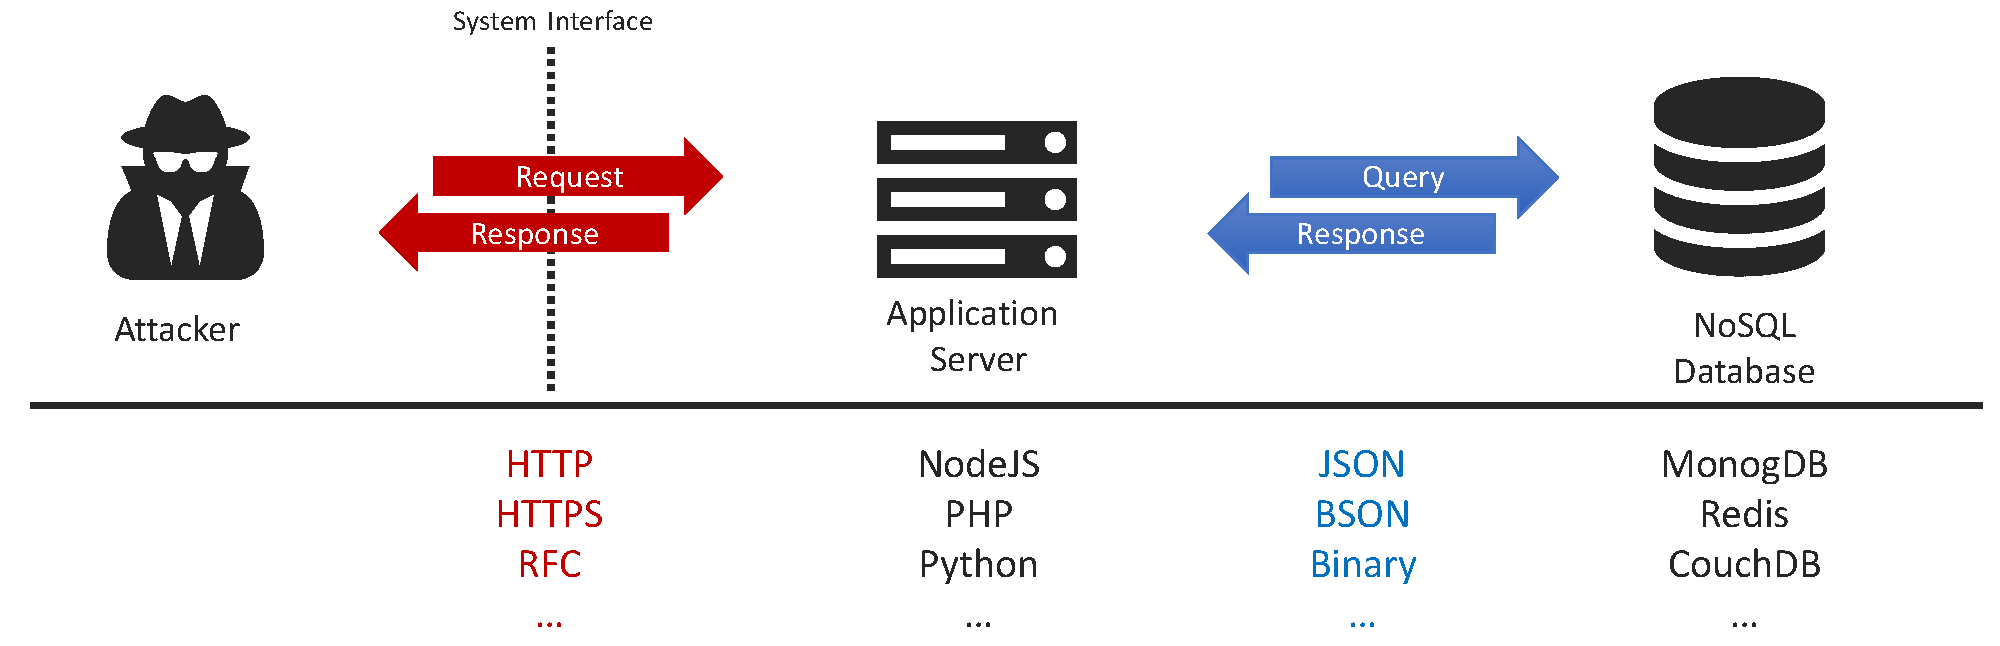
\includegraphics[width=1\linewidth]{Images/attacker_model_normal}
  \caption{Common attacker model for NoSQL injection}
  \label{fig:normalAttackerModel}
\end{figure}

% Objective

\subsection{Extended Attacker Model}

\begin{figure}[h]
\centering
  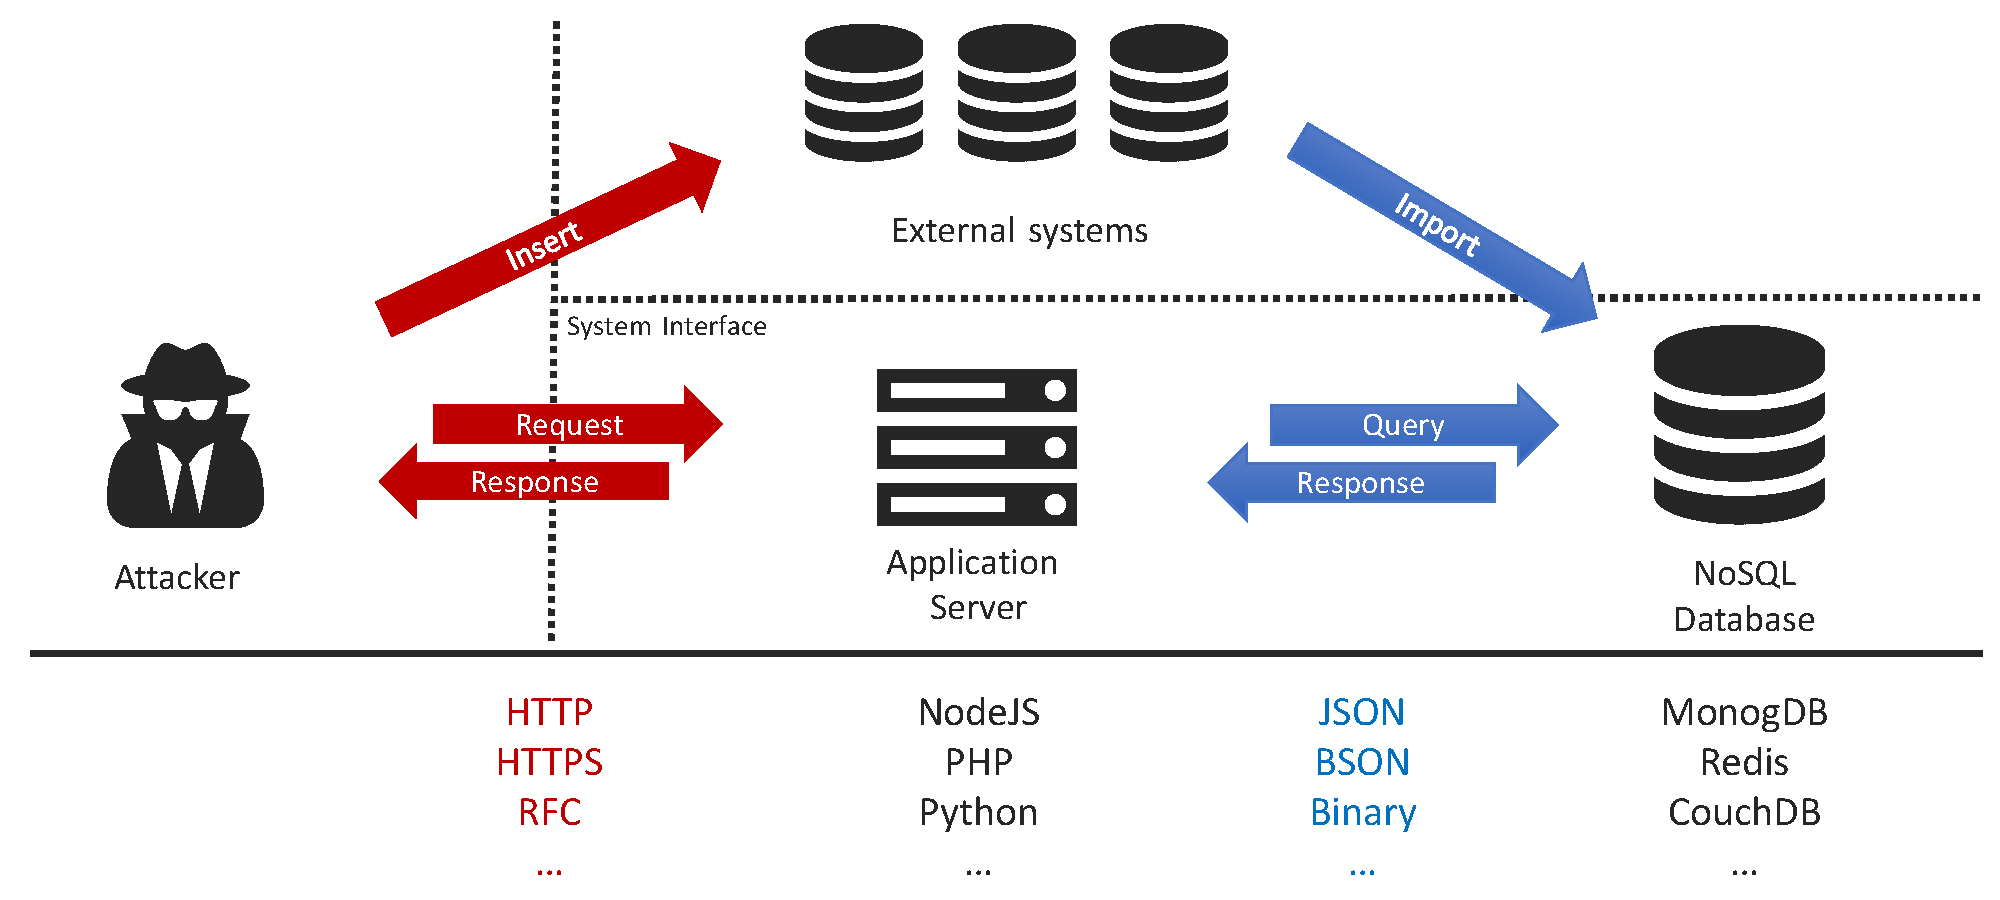
\includegraphics[width=1\linewidth]{Images/attacker_model_extended}
  \caption{Extended attacker model for NoSQL injection}
  \label{fig:extendedAttackerModel}
\end{figure}

% Objective

\subsection{Direct Attacker Model}

The deployment of RESTful interfaces allows a direct access from the client, omitting any application layer. Databases such as CouchDB explicitly refer to this architectural style for a simpler application design.

\begin{figure}[h]
\centering
  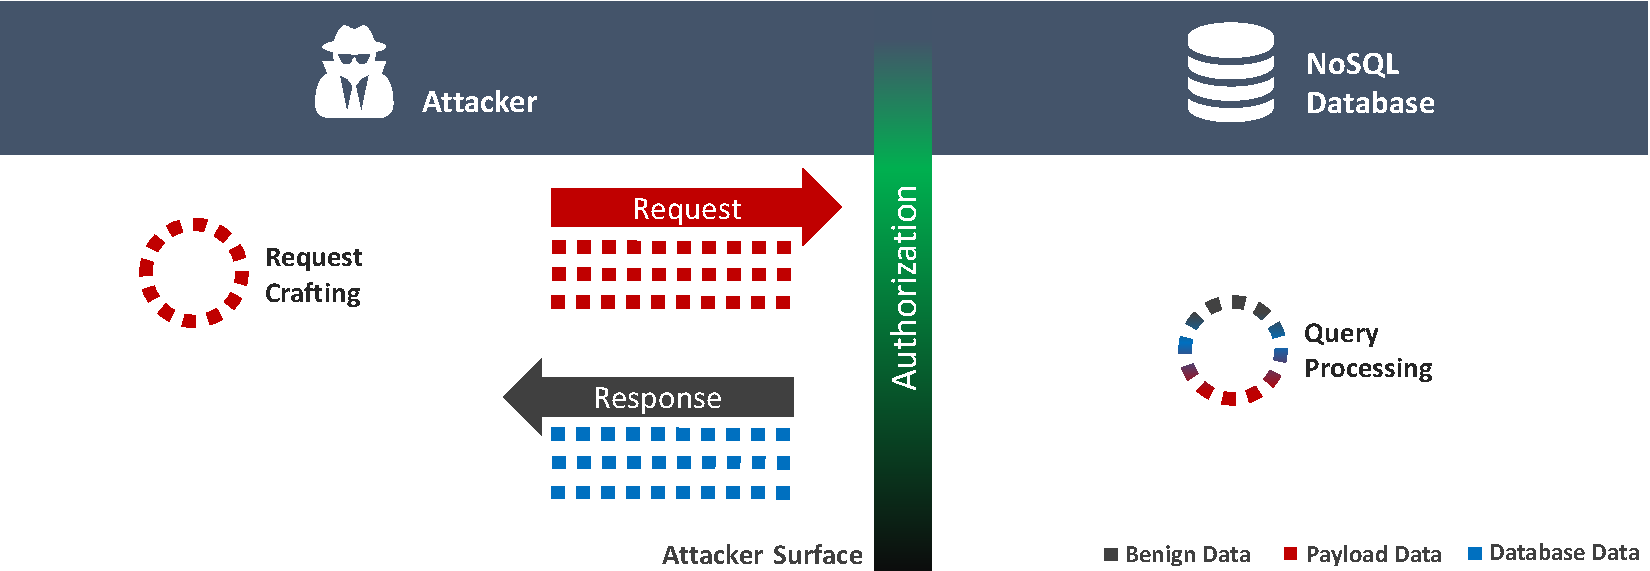
\includegraphics[width=1\linewidth]{Images/attacker_model_direct}
  \caption{Direct attacker model for NoSQL injection}
  \label{fig:extendedAttackerModel}
\end{figure}

% Objective


\section{Considered Technology Stack}
\subsection{Selected Databases}
\subsection{Selected Application Platforms}